%\documentclass{book}
\documentclass[10.5pt]{jarticle}
%\documentclass[11pt]{report}
%\usepackage{ramsstyle}

%\usepackage[dvips]{graphicx}
%\usepackage[draft,dvipdfmx]{graphicx, xcolor}
\usepackage{amsmath,amsthm,amssymb,bm}
\usepackage{url, braket, setspace}
\usepackage{latexsym}
\usepackage{booktabs}
\usepackage{tabularx}
\usepackage{float}
\usepackage{listings}
\usepackage{slashed}
\usepackage{hyperref}
\hypersetup{
    colorlinks,
    citecolor=blue,
    filecolor=blue,
    linkcolor=blue,
    urlcolor=blue
}

\usepackage{courier}

\usepackage{subfigure}
\usepackage{multirow}
\usepackage{lscape}
\usepackage{xspace}
\usepackage{rotating}
\usepackage{changepage}
\usepackage{booktabs} % M.G.                                                                                                                                                                              
\usepackage{verbatim}
\usepackage{sverb}
\usepackage{textcomp}
\usepackage{capt-of}
%

%
\setlength{\topmargin}{-1.5cm}
\setlength{\oddsidemargin}{-0.3cm}
\setlength{\evensidemargin}{-0.3cm}
\setlength{\textwidth}{16.5cm}
\setlength{\textheight}{23.7cm}
\setlength{\abovedisplayskip}{4pt} % upper margin
\setlength{\belowdisplayskip}{8pt}% lower margin
%
\newcommand{\nn}{\nonumber}
\newcommand{\beq}{\begin{align}}
\newcommand{\eeq}{\end{align}}
\newcommand{\colv}[1]{\left( \begin{array}{c} #1 \end{array} \right)}
\newcommand{\tab}[4]{\begin{table}[h] \begin{center} \caption{#3} \begin{tabular}{#1} #2 \end{tabular}  \label{#4} \end{center}   \end{table}}
\newcommand{\tabsmall}[4]{\begin{table}[h] \begin{center} \small \caption{#3} \begin{tabular}{#1} #2 \end{tabular}  \label{#4} \end{center}   \end{table}}
\newcommand{\tabtiny}[4]{\begin{table}[h] \begin{center} \tiny \caption{#3} \begin{tabular}{#1} #2 \end{tabular}  \label{#4} \end{center}   \end{table}}
%
\def \mm#1{\mathrm{#1}}
% fig 
\newcommand{\fig}[4][width=15cm]{
	\begin{figure}[H]
		 \centering
			 \includegraphics[width=#1mm]{figures/#2}
		 \caption{#3}
		 \label{#4}
	 \end{figure}} 
% fig (not H)
\newcommand{\figNoH}[4][width=15cm]{
	\begin{figure}
		 \centering
			 \includegraphics[width=#1mm]{figures/#2}
		 \caption{#3}
		 \label{#4}
	 \end{figure}} 
 % Math
 \newcommand{\MP}[1]{\mbox{\phantom{#1}}}
 \newcommand{\der}[1]{d #1}
 \newcommand{\mcal}{\mathcal{M}}
 \newcommand{\ddt}{\frac{\mathrm{d} }{\mathrm{d} t}}
 \newcommand{\pdt}{\frac{\partial }{\partial t}}
%
 \newcommand{\intlumi}{36.1 $\mathrm{fb}^{-1}$}
%
\newcommand{\tev}{\, \mathrm{TeV}}
\newcommand{\gev}{\, \mathrm{GeV}}
\newcommand{\mev}{\, \mathrm{MeV}}
\newcommand{\um}{\mathrm{\mu m}}
\newcommand{\us}{\mathrm{\mu s}}
\newcommand{\cdeg}{{}^\circ\mathrm{C}}
%
\newcommand{\ra}{\rightarrow}
\newcommand{\ua}{\uparrow}
\newcommand{\da}{\downarrow}
\newcommand{\ol}{\overline}
\newcommand{\dg}{\dagger}
% 3-vectors
\newcommand{\bp}{\bm{p}}
\newcommand{\bn}{\bm{n}}
\newcommand{\bnn}{\bm{n'}}
\newcommand{\bmet}{\bm{\slashed{E}_{\mathrm{T}}}}
\newcommand{\bpt}{\bm{p}_{\mathrm{T}}}
% sin/cos
\newcommand{\costh}{\cos{\theta}}
\newcommand{\sinth}{\sin{\theta}}
\newcommand{\costhh}{\cos{\frac{\theta}{2}}}
\newcommand{\sinthh}{\sin{\frac{\theta}{2}}}
\newcommand{\costthh}{\cos^2{\frac{\theta}{2}}}
\newcommand{\sintthh}{\sin^2{\frac{\theta}{2}}}
%
\newcommand{\ltsim}{\protect\raisebox{-0.5ex}{$\:\stackrel{\textstyle <}{\sim}\:$}} % <~
\newcommand{\gtsim}{\protect\raisebox{-0.5ex}{$\:\stackrel{\textstyle >}{\sim}\:$}} % >~
\newcommand{\ltsimscript}{\protect\raisebox{-0.5ex}{$\stackrel{\scriptstyle <}{\sim}$}} % <~
\newcommand{\gtsimscript}{\protect\raisebox{-0.5ex}{$\stackrel{\scriptstyle >}{\sim}$}} % >~

%
% SUSY aliases
\newcommand{\mMSSM}{\mathrm{MSSM}}
\newcommand{\mSM}{\mathrm{SM}}
\newcommand{\mGUT}{\mathrm{GUT}}
\newcommand{\mup}{\mathrm{u}}
\newcommand{\mdn}{\mathrm{d}}
\newcommand{\mL}{\mathrm{L}}
\newcommand{\mR}{\mathrm{R}}
\newcommand{\tQ}{\tilde{Q}}
\newcommand{\tL}{\tilde{L}}
%
\newcommand{\te}{\tilde{e}}
\newcommand{\tebar}{\tilde{\bar{e}}}
\newcommand{\tu}{\tilde{u}}
\newcommand{\tubar}{\tilde{\bar{u}}}
\newcommand{\td}{\tilde{d}}
\newcommand{\tdbar}{\tilde{\bar{d}}}
\newcommand{\ttop}{\tilde{t}}
\newcommand{\tb}{\tilde{b}}
\newcommand{\ttau}{\tilde{tau}}
\newcommand{\tlep}{\tilde{\ell}}
%
\newcommand{\chaone}{\tilde{\chi}_{1}^{\pm}}
\newcommand{\tchic}{\tilde{\chi}_{1}^{\pm}}
\newcommand{\tchin}{\tilde{\chi}_{2}^{0}}
\newcommand{\tLSP}{\tilde{\chi}_{1}^{0}}
\newcommand{\neutwo}{\tilde{\chi}_{2}^{0}}
%
\newcommand{\tH}{\tilde{H}}
\newcommand{\tW}{\tilde{W}}
\newcommand{\tB}{\tilde{B}}
\newcommand{\tg}{\tilde{g}}
\newcommand{\mG}{m_{\tg}}
%\newcommand{\mG}{m(\tilde{g})}
\newcommand{\mC}{m_{\tchic}}
\newcommand{\mN}{m_{\tchin}}
\newcommand{\mCN}{m_{\tchic/\tchin}}
\newcommand{\mLSP}{m_{\tLSP}}
\newcommand{\dmg}{\Delta m(\tg, \, \tLSP)}
\newcommand{\dmcn}{\Delta m(\tchic/\tchin, \, \tLSP)}
\newcommand{\dmc}{\Delta m(\tchic, \, \tLSP)}
\newcommand{\dmn}{\Delta m(\tchin, \, \tLSP)}


%
% Process names
\newcommand{\wjets}{W+\mathrm{jets}}
\newcommand{\zjets}{Z+\mathrm{jets}}
\newcommand{\vjets}{V+\mathrm{jets}}
\newcommand{\wzjets}{W/Z+\mathrm{jets}}
\newcommand{\ttbar}{t\bar{t}}
\newcommand{\vvjets}{VV+\mathrm{jets}}
\newcommand{\mislep}{\slashed{\ell}}
\newcommand{\llmis}{\ell\mislep}
\newcommand{\ltauh}{\ell\tau_h}
\newcommand{\ttbarFakeB}{\ttbar+b_{\mathrm{fake}}}

% stats
\newcommand{\clsb}{\mathrm{CL}_{s+b}}
\newcommand{\clb}{\mathrm{CL}_b}
\newcommand{\cls}{\mathrm{CL}_s}
\newcommand{\musig}{\mu_{\mathrm{sig.}}}
\newcommand{\mutop}{\mu_{\mathrm{Top}}^i}
\newcommand{\muw}{\mu_{\mathrm{W}}^i}
\newcommand{\SR}{\mathrm{SR}}
\newcommand{\TR}{\mathrm{TR}}
\newcommand{\WR}{\mathrm{WR}}
\newcommand{\CR}{\mathrm{CR}}
\newcommand{\bmtheta}{\bm{\theta}}

% Generators
\newcommand{\sherpa}{\SHERPA}
\newcommand{\sherpatwo}{\SHERPA 2.2.1}
\newcommand{\powheg}{\POWHEG}
\newcommand{\powhegbox}{\POWHEG+Box}
\newcommand{\mgmc}{MG5\_aMC@NLO}
\newcommand{\pythia}{\PYTHIA}
\newcommand{\pythiasix}{\PYTHIA 6.428}
\newcommand{\pythiaeight}{\PYTHIA 8.186}
\newcommand{\herwig}{\HERWIG}


\newcommand{\antikt}{anti-$k_{\mathrm{T}}$}
\newcommand{\Antikt}{Anti-$k_{\mathrm{T}}$}

% gridname
\newcommand{\dire}{\texttt{Direct} }
\newcommand{\xhalf}{\texttt{x=1/2} }
\newcommand{\varx}{\texttt{LSP60} }
\newcommand{\DMtw}{\texttt{DM20} }
\newcommand{\DMth}{\texttt{DM30} }




% kinematical variables
\newcommand{\DR}{\Delta R}
\newcommand{\ppp}{p_{\mathrm{\perp}}}
\newcommand{\ttPt}{\pt(\ttbar)}
\newcommand{\met}{E_{\mathrm{T}}^{\mathrm{miss}}}
\newcommand{\meffInc}{m_{\mathrm{eff}}}
\newcommand{\meffIncFirst}{m_{\mathrm{eff}}^{\mathrm{bin 1}}}
\newcommand{\meffIncSecond}{m_{\mathrm{eff}}^{\mathrm{bin 2}}}
\newcommand{\meffIncThird}{m_{\mathrm{eff}}^{\mathrm{bin 3}}}
\newcommand{\nLepbase}{n_{\ell, \mathrm{base.}}}
\newcommand{\nLepsignal}{n_{\ell, \mathrm{sig.}}}
\newcommand{\nJetNoGev}{n_{\mathrm{jet}}}
\newcommand{\nBJetNoGev}{n_{\mathrm{b-jet}}}
\newcommand{\nJet}{n_{\mathrm{J}} \,(p_{\mathrm{T}}>30\gev)}
\newcommand{\fourthJetPt}{\pt(j_4)}
\newcommand{\nBJet}{n_{\mathrm{B}} \, (p_{\mathrm{T}}>30\gev)}
\newcommand{\lepOnePt}{p_{\mathrm{T}}(\ell_1)}
\newcommand{\lepTwoPt}{p_{\mathrm{T}}(\ell_2)}
\newcommand{\lepPt}{p_{\mathrm{T}}(\ell)}
\newcommand{\wpt}{p_{\mathrm{T}}(W)}
\newcommand{\mtFull}{m_{\mathrm{T}} (\lepPt, \met) }
\newcommand{\mtRep}{\mt(\ell_{\mathrm{rep.}},\met) }
\newcommand{\mt}{m_{\mathrm{T}} }
\newcommand{\mindPhiFourJet}{\displaystyle \min_{i=1-4} \Delta \phi(j_i, \met)}
\newcommand{\LepAplanarity}{\mathrm{Aplanarity}}
\newcommand{\apl}{\mathrm{aplanarity}}
\newcommand{\Apl}{\mathrm{Aplanarity}}
\newcommand{\topNess}{\mathrm{Topness}}
\newcommand{\metOverMeff}{\met/\meffInc}
\newcommand{\nJetOverLepPt}{\nJetNoGev/\lepPt}

\newcommand{\etcone}{\ET^{\mathrm{cone\,\,0.2}} }
\newcommand{\ptcone}{\pt^{\mathrm{cone\,\,0.2}} }



%
\begin{document}
\bibliographystyle{unsrt}

%%\documentclass {article}
\setlength{\topmargin}{-1.5cm}
\setlength{\oddsidemargin}{-0.3cm}
\setlength{\evensidemargin}{-0.3cm}
\setlength{\textwidth}{16.5cm}
\setlength{\textheight}{23cm}
%\usepackage{graphicx}
%\usepackage{float}
%\usepackage{url, braket, setspace}
%\usepackage{amsmath,amsthm,amssymb,bm}
%\usepackage{hyperref}


%\begin{document}

\topmargin =-20mm
\title{Search for Gluinos using Final States with One Isolated Lepton in the LHC-ATLAS Experiment.}
\author{Shion Chen \thanks{chen@icepp.s.u-tokyo.ac.jp} \\ \\
\fontsize{10.0pt}{0pt}\selectfont Department of Physics, Graduate School of Science, The University of Tokyo\\
\fontsize{10.0pt}{0pt}\selectfont 7-3-1, Hongo, Bunkyo-ku, 113-0033, Tokyo, Japan }
%
\date{}

\maketitle

\begin{center}
%\textbf{Abstract} \\
\begin{figure}
\begin{center}
%�
\includegraphics[width=3cm]{./figure/UTlogo.eps}
\end{center}
\end{figure}

\end{center}

\clearpage

\begin{center}
%\textbf{Abstract} \\
\begin{figure}
\begin{center}

\includegraphics[width=3cm]{./figures/UTlogo.eps}
\end{center}
\end{figure}

\end{center}

\clearpage

\topmargin =-13mm

%\tableofcontents





%\end{document}

\pagenumbering{roman}
\setlength{\baselineskip}{15pt}
%\newpage
\pagenumbering{arabic}
%
%



%\documentclass {article}
\setlength{\topmargin}{-1.5cm}
\setlength{\oddsidemargin}{-0.3cm}
\setlength{\evensidemargin}{-0.3cm}
\setlength{\textwidth}{16.5cm}
\setlength{\textheight}{23cm}
%\usepackage{graphicx}
%\usepackage{float}
%\usepackage{url, braket, setspace}
%\usepackage{amsmath,amsthm,amssymb,bm}
%\usepackage{hyperref}


%%%%%%%%%%%%

%\begin{document}

%\section*{Abstract} 
%\paragraph{Search for Gluinos using Final States with One Isolated Lepton in the LHC- ATLAS Experiment \mbox{\phantom{MMMMMM}} Shion Chen}


\begin{center}
論文要旨
\end{center}

This thesis presents the search for gluinos via proton-proton collisions with the center-of-mass energy of $\sqrt{s}=13\tev$ at Large Hadron Collider (LHC), through examining the final state with exactly one leptons.  \\

%Despite the enormous success of the Standard Model in particle physics, there are still quite a room for unrevealed mysteries of universe;
Despite the enormous success of the Standard Model (SM) in particle physics, there are still a number of problems left to be solved such as the problem of diverging higgs mass and the unaccounted presence of dark matter and so on.
%as well as for the persue toward the ``theoy of everything'' with grand unification and gravity.
It is then strongly motivated to extend the Standard Model, and the Minimal Supersymmetric Standard Model (MSSM) has been one of the most applealing candidates, introducing a boson-fermion symmetry (super-symmetry; SUSY). 
SUSY theories generally predict another set of particle contents with respect to SM, with the masses potentially accessible by experiments.
Numerous experiments have been performed searching for SUSY particles both directly or indirectly.
Though no evidence has been claimed ever, searches in the LHC are still highly motivated since it allows to probe heavier regions with the unprecedented high center-of-mass energy with increased data statistics.
Gluino search is particularly interesting due to the large production cross-section that fully exploits the merit of hadron collider, as well as absence of theoretical or experiments constrains. \\
%The motivation of gaugino search is increasingly emerging in light of the discovery of higgs boson in its mass of $125\gev$, and gluino search is particularly interesting due to the large production in LHC.   \\

This thesis presents the search for gluinos via proton-proton collisions with the center-of-mass energy of $\sqrt{s}=13\tev$ at LHC, by focusing on the final state with exactly one leptons. 
Using the improved analysis technique and increased data with 36.1 fb$^{\-1}$ of integrated luminosity collected in the ATLAS detector, the sensitivity to heavier gluino is drastically gained.  \\
%\cite{fineTuning}

In this analysis, the main improvement with respect to past searches are two-fold: 
\begin{itemize}
\item Widen the scope of search in terms of variety of gluino decay chains and the scenario of SUSY mass spectra.
The one problem in the past search was that only a few typical gluino decays have been studied, while a number of decays remain uncovered.
In this new analysis, we started from the most general cases by considering all the possible gluino decays, and converge into 45 chains that could give different kinematical behavior.
Constraint is studied for all the 45 decay chains. In addition, we also focus on a scenario generally motivated by observed relic of dark matter where the lightest two EW gauginos have the masses comppressed.
Signal regions are segmented with 18 different bins to address all the decay models, with particular attention to paid on cut optimization reconsiling the inclusiveness and sensitivity. \\


\item An introduction of a dedicated data-driven strategy of background estimation.
One general characteristic of new physics search is that it has to focus on an extreme phase space that is often ill-modeled by MC simulation due to the sizable contribution from higher orer pertuabation.
In this analysis, a combination of semi-data driven method in which the MC prediction is corrected in a set of control regions, and a fully data-driven ``object replacement method'' 
where one of the lepton in 2-lepton region is replaced into virtual mis-identified lepton or tau, estimating the yield resulting in 1-lepton regions including the signal regions.
The estimation is shown to be more robust compared with conventional simulation-based method. \\
\end{itemize}



\fig[160]{histpull_SRs.eps}
{Expected background level (colored stack) and observed number of data events in the 18 signal region bins.}
{SRpull}


%%%%%%%%%%
\begin{figure}[h]
  \centering
    \subfigure[]{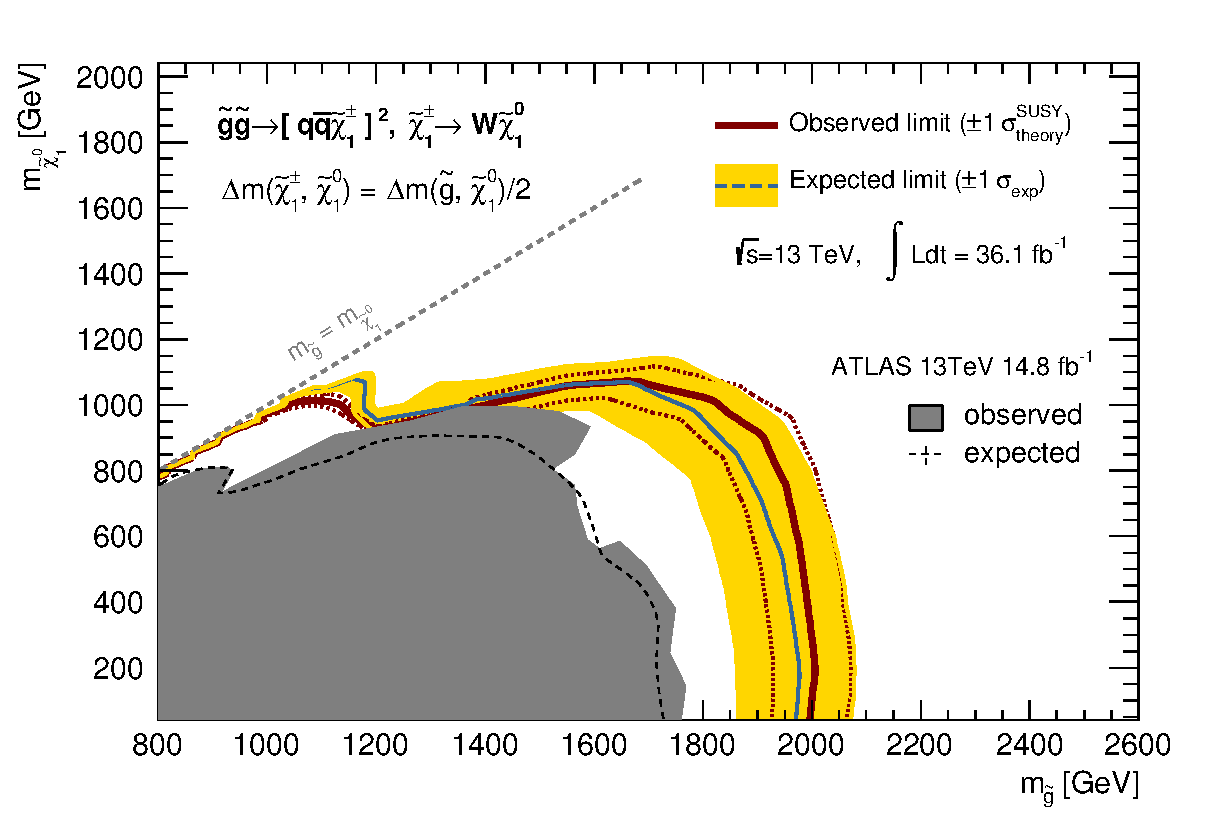
\includegraphics[width=0.48\textwidth]{figures/excl_GG_symQQC1_fixSigXSecNominal_x12.eps}}
    \subfigure[]{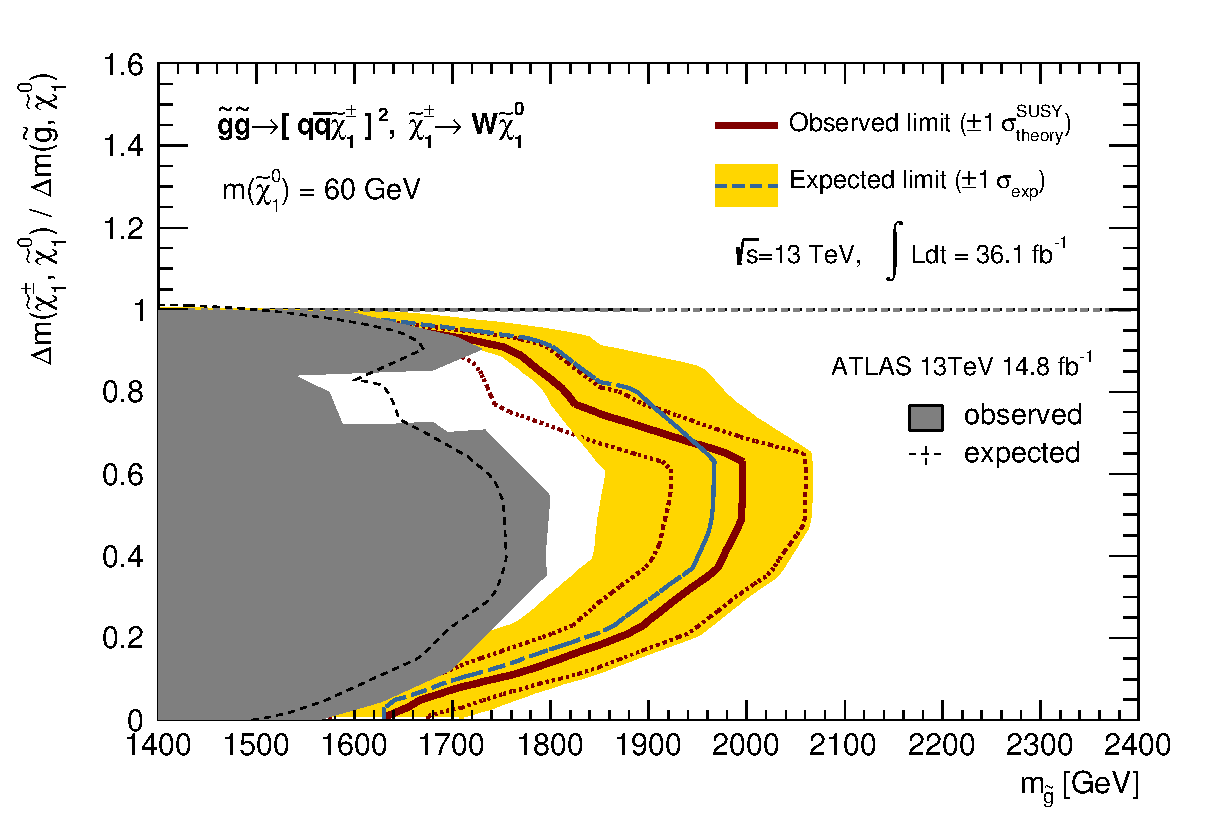
\includegraphics[width=0.48\textwidth]{figures/excl_GG_symQQC1_fixSigXSecNominal_varx.eps}}
    \caption{ Exclusion limits obtained by the analysis on the reference model ($pp \ra \tg\tg,  \tg \ra q\bar{q} \tchic$) shown 
  (a) in the $m_{\tg}-m_{\tLSP}$ plane where the mass of the intermediate chargino is set to the midmost between gluino and the lightest neutralino, or either 
  (b) in the $m_{\tg}-x$ plane where $x:= (m_{\tchic}-m_{\tLSP})/(m_{\tg}-m_{\tLSP})$ and the lightest neutralino mass is set to $m_{\tLSP}=60\gev$. 
  The limit set by up-to-date precious search \cite{2016ICHEP} is indicated by the grey shade.
  \label{limit_symQQC1} }
\end{figure}
%%%%%%%%%%


\fig[160]{3B_x12_obs.eps}
{Observed exclusion limits on gluino decay chains targeted by the 3 b-tagged signal regions overlaid on a single plane. 
For models involving an intermediate EW gaugino, the mass is set to the midmost between gluino and the lightest neutralino.}
{combLimit}

No significant excess is found in the unblinded dataset as shown in Figure \ref{SRpull}, and exclusion limits are set on wide range of gluino decay scenarios. 
The limit on process $pp \ra \tg\tg,  \tg \ra q\bar{q} \tchic$ is presented in Figure \ref{limit_symQQC1}, which has been commonly used as benchmark in past analysis.
The limit extends about $100-300\gev$ by the increased dataset together with improved analysis, hitting nearly $2\tev$ in gluino mass. 
Various other cases are also examined (part of them are shown in Figure \ref{combLimit}), and as a general conclusion, 
it is confirmed that up to $1.7\tev - 2.0 \tev$ in gluino mass and up to $\sim 1\tev$ in the lightest neutralino mass is excluded for typical mass spectra, 
while the limit extends up to $1.5\tev - 1.9 \tev$ in gluino mass in case of compressed EW gaugino masses ($\Delta M \sim 20-30\gev$) that is motivated by dark matter relic observations.


%%%%%%%%%%%%%%%%%%%%%%%%%%%%%%%%%%%%%%%%%%%%%%%
\begin{thebibliography}{99}
%\bibitem {fineTuning}  L. J. Hall, D. Pinner, and J. T. Ruderman, ``A Natural SUSY Higgs Near 126 GeV'', JHEP 04 (2012) 131, arXiv:1112.2703 [hep-ph].
\bibitem {2016ICHEP} ATLAS Collaboration, ``Search for squarks and gluinos in events with an isolated lepton, jets and missing transverse momentum at √s = 13 TeV with the ATLAS detect'' ATLAS-CONF-2016-054 (2016).
%\bibitem {DM} 
\end{thebibliography}

%\end{document}





\end{document}
